\documentclass[11pt,a4paper]{article}

\usepackage{style2017}
\usepackage{hyperref}

\hypersetup{
    colorlinks =false,
    linkcolor=blue,
   linkbordercolor = 1 0 0
}
\newcounter{numexo}
\setcellgapes{1pt}

\begin{document}



\begin{NSI}
{TP}{Les fractales}
\end{NSI}

La programmation se fera avec un éditeur dédié comme pyzo ou thonny puisqu'il nécessite l'utilisation de la bibliothèque Turtle qui lance une fenêtre d'affichage.

Le fichier programme python sera nommé fractales.py

\section{Présentation}

Une figure fractale ou fractale est une courbe ou surface de forme irrégulière ou morcelée qui se
crée en suivant des règles déterministes ou stochastiques impliquant une homothétie interne. Le
terme « fractale » est un néologisme créé par Benoît Mandelbrot en 1974 à partir de la racine latine
fractus, qui signifie brisé, irrégulier .
Un des plus beaux exemples de fractale donné par la nature est le chou Romanesco (à gauche):

\begin{center}
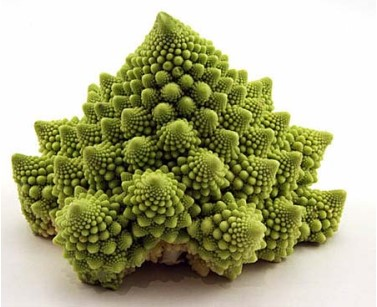
\includegraphics[scale=1]{img/chou.eps}\hspace{1cm}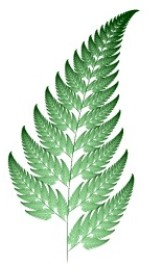
\includegraphics[scale=1]{img/fougere.eps}
\end{center}
Si l'on ne regarde qu'une des pointes, on a l'impression de voir un chou en entier. C'est le principe
d'auto-similarité. On retrouve de l'auto-similarité dans les fougères (à droite) : chaque feuille
ressemble à la fougère entière.


\section{La courbe du dragon}
La courbe du dragon (ou « Fractale du dragon » ou « courbe de Heighway » ou « dragon de
Heighway ») a été pour la première fois étudiée par les physiciens de la NASA John Heighway,
Bruce Banks, et William Harter. Elle a été décrite par Martin Gardner dans sa chronique de jeux
mathématiques du Scientific American en 1967. Nombre de ses propriétés ont été publiées par
Chandler Davis et Donald Knuth.

La courbe du dragon se construit ainsi:
\begin{center}
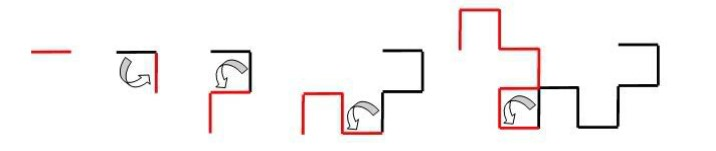
\includegraphics[scale=0.8]{img/courbe_dragon.eps}
\end{center}

\begin{itemize}
\item Si n = 0, on dessine une ligne. C'est la base (ou l'initiateur). La longueur a peu
d'importance. On définit la longueur une fois avec un paramètre.
\item Sinon, si n > 0 :
\begin{itemize}
\item Dragon (n-1)
\item On tourne à 90 degrés
\item Dragon (n-1). 
\end{itemize}
C'est la règle de récursivité (ou le générateur).
\end{itemize}

\begin{enumerate}
\item Programmer cette fractale pour la représenter avec le la librairie Turtle.
\item Dessiner cette fractale. Que remarquez-vous ?
\item Pour obtenir une fractale correcte, il faut introduire une rotation de -90 degrés. L'astuce consiste à passer un second paramètre s dans la fonction qui prendra comme valeur 1 ou -1 et on multiplie l'angle de rotation par s. Modifier votre programme en conséquence.

La figure ci-dessous représente une fractale du dragon pour n=8.
\begin{center}
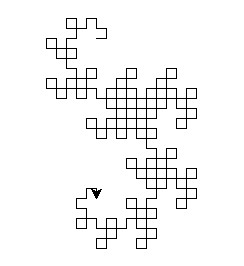
\includegraphics[scale=1]{img/fractale_dragon.eps}
\end{center}
\end{enumerate}

\section{Le flocon de von Koch}

Le flocon de von Koch est l'une des premières courbes fractales à avoir été décrite (bien avant l'invention du terme « fractal(e) »). Elle a été inventée en 1906 par le mathématicien suédois Helge von Koch.

La courbe de von Koch se réalise à patir d'un segment de droite, en modifiant récursivement chaque segment de droite de la façon suivante :
\begin{enumerate}
\item On divise le segment de droite en trois segments de longueurs égales.
\item On dessine les 4 morceaux de segments de longueur le tiers du segment en effectuant des rotations pour obtenir la forme.
\item on recommence le processus sur chacun des 4 morceaux de segments.
\end{enumerate}\medskip

\begin{minipage}{12cm}
Au bout de ces trois étapes, l'objet résultant a une
forme similaire à une section transversale d'un chapeau de
sorcière. La courbe de von Koch est la limite des courbes
obtenues, lorsqu'on répète indéfiniment les étapes
mentionnées ci-avant.\medskip

\end{minipage}\hfill
\begin{minipage}{6cm}
\begin{center}
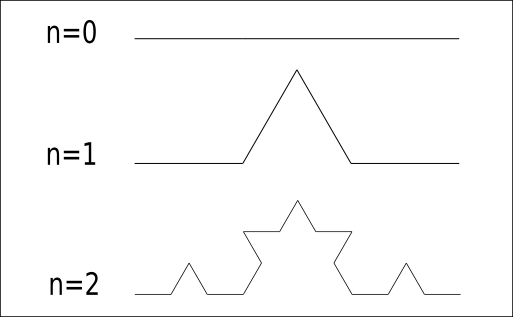
\includegraphics[scale=0.4]{img/courbe_van_koch.eps}
\end{center}
\end{minipage}

\begin{minipage}{12cm}
Le \textbf{flocon de von Koch} s'obtient de la même façon que
la fractale précédente, en partant d'un triangle équilatéral
au lieu d'un segment de droite, et en effectuant les
modifications en orientant les triangles vers l'extérieur.
\end{minipage}\hfill
\begin{minipage}{6cm}
\begin{center}
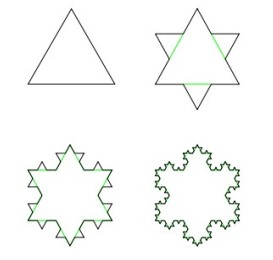
\includegraphics[scale=0.6]{img/flocon_van_koch.eps}
\end{center}
\end{minipage}
\begin{enumerate}
\item La fonction \textbf{courbe\_van\_koch(n,l)} prend en paramètre le nombre de répétitions du modèle obtenu lorsque n=1 et la longueur initiale l du segment. Cette fonction dessine la courbe de Van Koch.
\item Écrire une fonction qui dessine le \textbf{flocon de Van Koch} à partir d'un triangle équilatéral.
\item Récrire vos deux fonctions en y apportant les modifications nécessaires pour que le modèle initial ressemble à la figure suivante:
\begin{center}
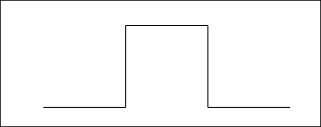
\includegraphics[scale=0.6]{img/carre_van_koch.eps}
\end{center}
\item Réaliser une fractale avec n=5.
\item Construire une figure superposant les fractales pour n=0 jusqu'à n=5 (figure ci-dessous).
\begin{center}
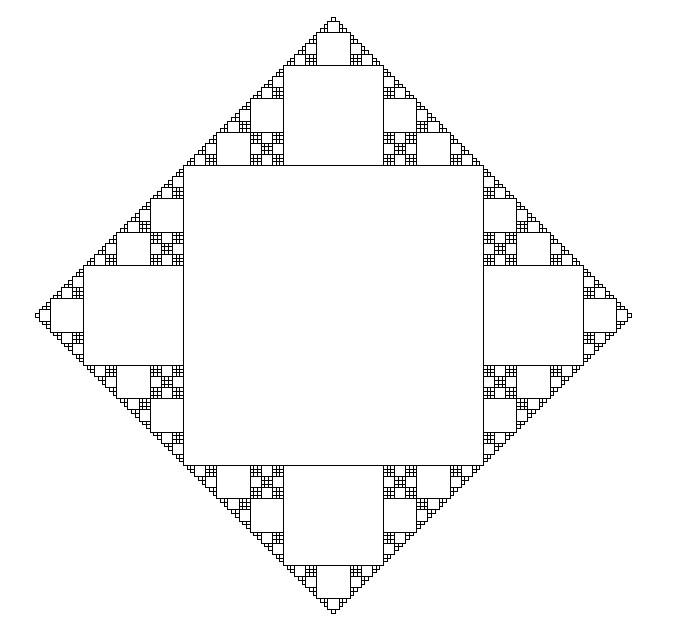
\includegraphics[scale=0.6]{img/carre_fractale_5.eps}
\end{center}
\end{enumerate}

\section{L'arbre}

Reproduire cette fractale arborescente avec un niveau de récursivité égal à 5. Le motif initial est un Y.
\begin{center}
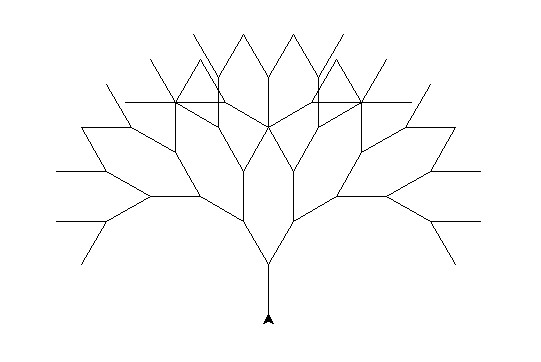
\includegraphics[scale=0.6]{img/arbre_fractale.eps}
\end{center}
Voici quelques indications :
\begin{itemize}
\item Commencer par les 3 premiers arbres sont représentés ci-dessous:
\begin{center}
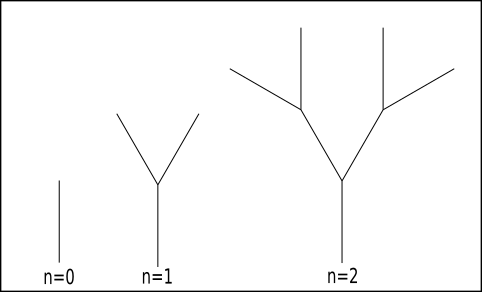
\includegraphics[scale=0.6]{img/arbre.eps}
\end{center}
\item Les angles de rotation sont de 30 degrés.
\item Une fois le tracé d'un trait réalisé, il faut revenir en arrière avec la commande \textbf{backward()}
\end{itemize}
\end{document}
